\chapter{Ansatz}\label{ch:ansatz}
Before we delve into details let us preface this section with an etymology of the word ansatz. In physics and mathematics, an ansatz (plural ansätze) is a German word that means an educated guess, an initial point, or an additional assumption made to help solve a problem, and which may later be verified to be part of the solution by its results \cite{ansatz_etymology}.

In the context of quantum computing, an ansatz is a parametrized quantum circuit,  a quantum circuit comprised of quantum gates and some of them are parametrized. Parametrized quantum circuits are often used in variational algorithms where the parameters are optimized by classical computers.

In this chapter, we will discuss the importance of the ansatz, its properties, and types. We will also introduce some popular ansatzes.

\section{Expressibility}
The notion of expressibility can be very helpful to get an understanding what is the role of the ansatz. Expressibility says how much of the Hilbert space can be covered by our ansatz. The following pictures should illustrate this concept very well.

\begin{figure}[H]
        \centering
        \begin{minipage}{0.4\linewidth}
            \centering
            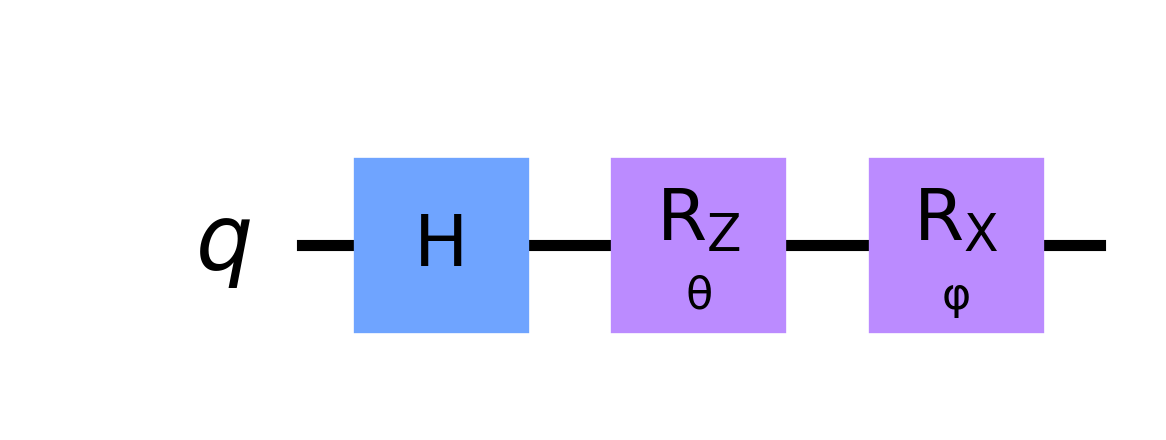
\includegraphics[width=\linewidth]{expressibility-hrzrx-circuit.png}
            \vfill
        \end{minipage}
        \hfill
        \begin{minipage}{0.4\linewidth}
            \centering
            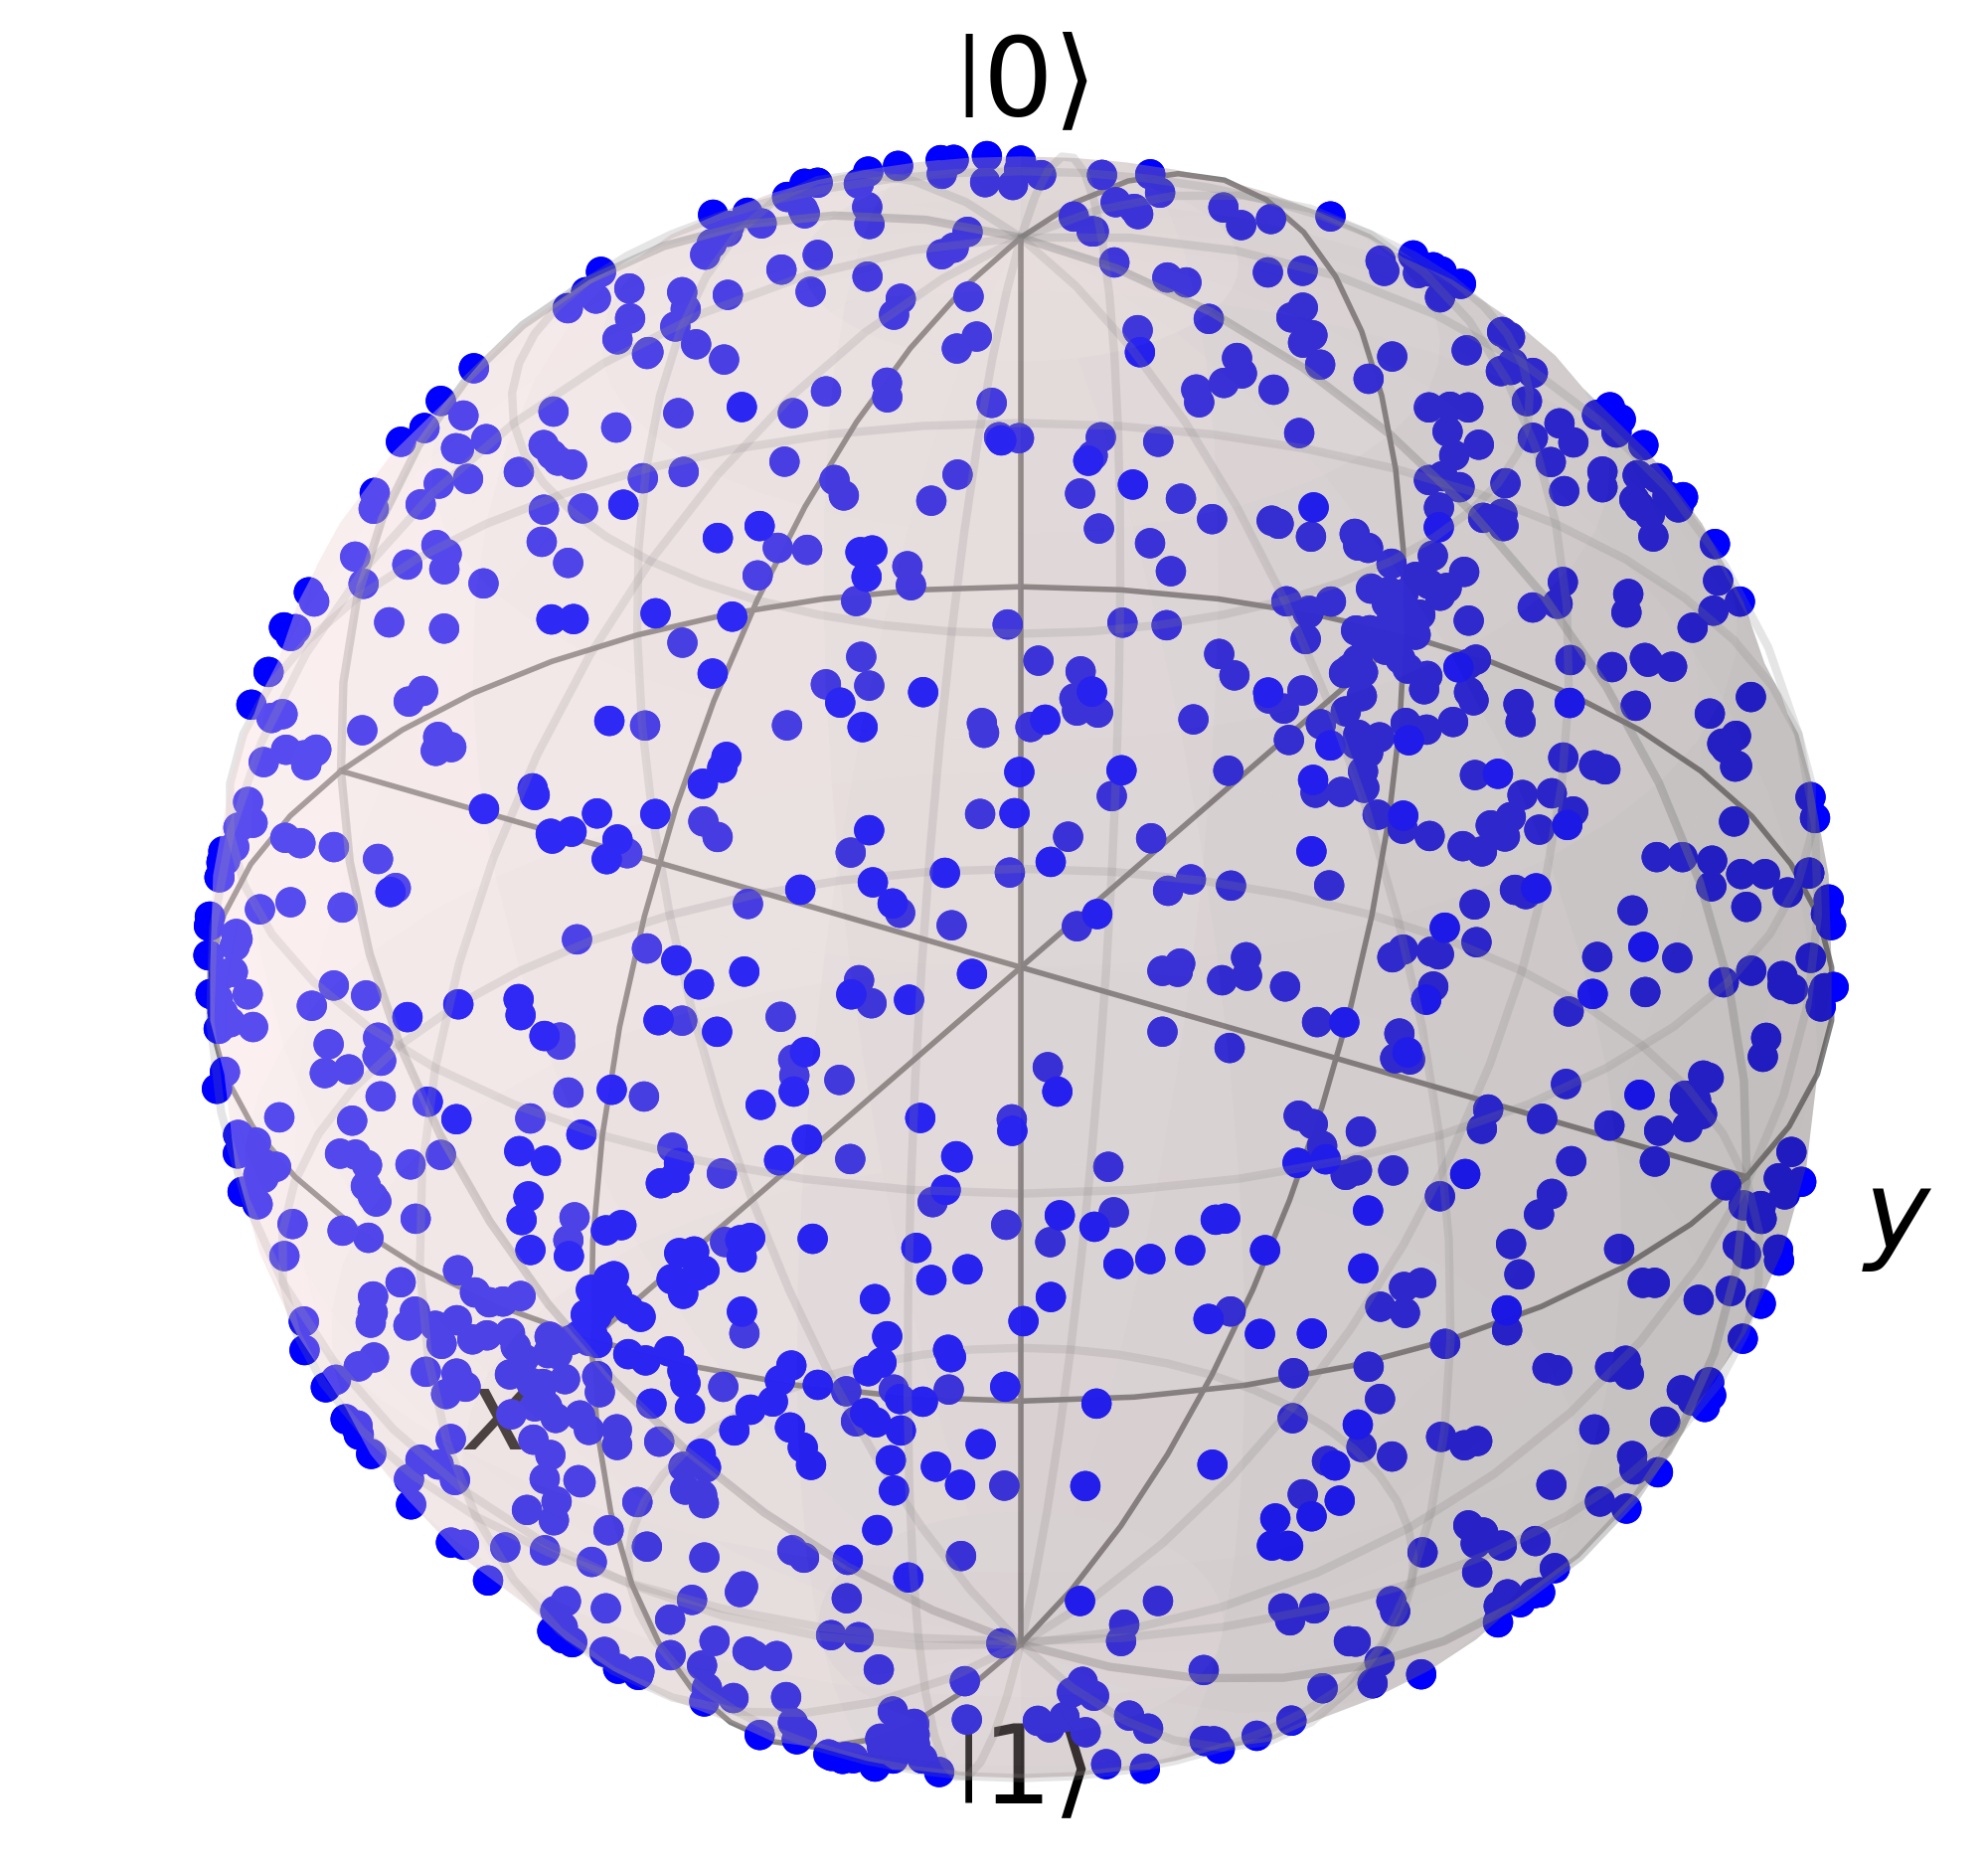
\includegraphics[width=\linewidth]{expressibility-hrzrx-qubit.png}
            \vfill
        \end{minipage}
        \caption{1000 points sampled uniformly randomly}
\end{figure}

Provided we know that our solution lies in the real part of Hilbert space, we can just use a simpler ansatz that covers only the real part of Hilbert space. Other gates would just introduce more noise to our circuit and the more parameters we have, the more difficult it is to optimize them.

\begin{figure}[H]
    \centering
    \begin{minipage}{0.4\linewidth}
        \centering
        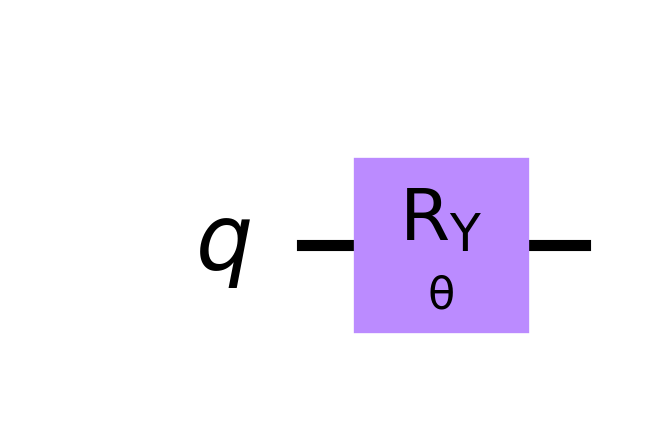
\includegraphics[width=\linewidth]{expressibility-ry-circuit.png}
        \vfill
    \end{minipage}
    \hfill
    \begin{minipage}{0.4\linewidth}
        \centering
        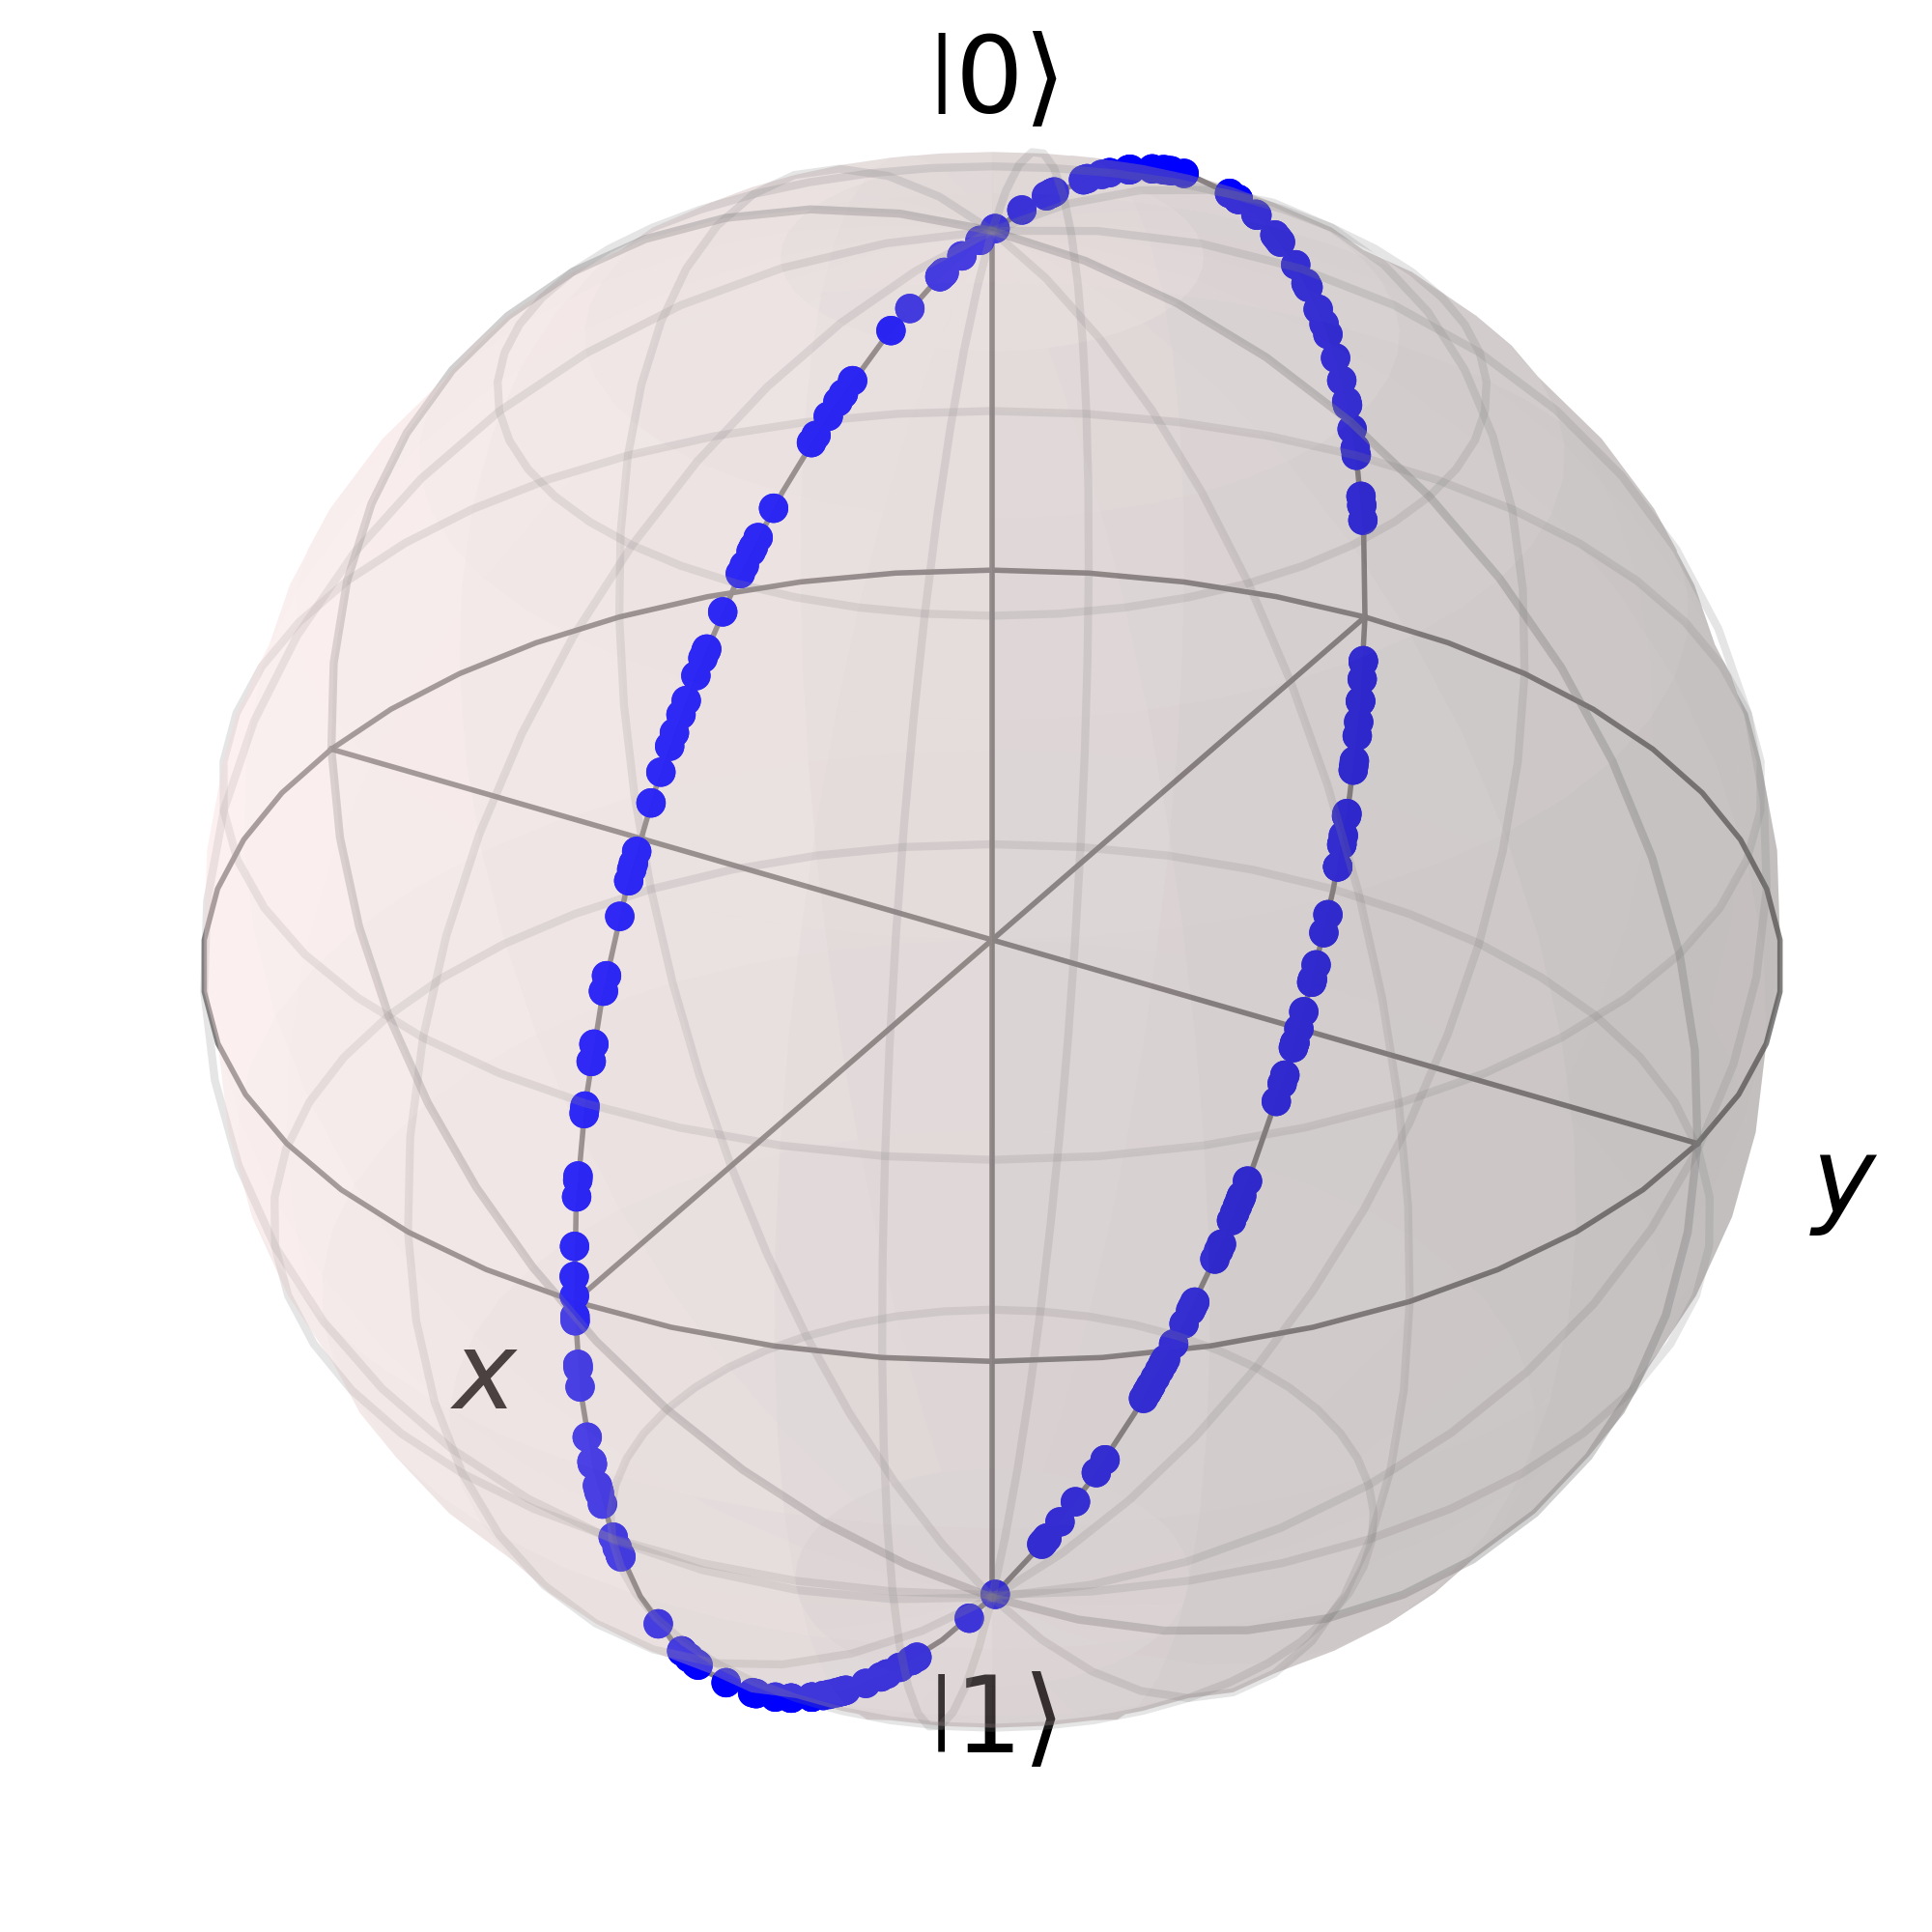
\includegraphics[width=\linewidth]{expressibility-ry-qubit.png}
        \vfill
    \end{minipage}
    \caption{200 points sampled uniformly randomly}
\end{figure}
\todo{make sure that the pictures circuit are of the same size}\\
\todo{should I include how to measure it? KL divergence?}


\section{Trainability}
Trainability refers to a process of how easy it is to find optimal parameters for our circuit. Circuit with higher amounts of qubits and parameters may exhibit problems with finding the optimal parameters. In the area of quantum circuits, it is mainly caused by the barren plateau (vast planes) problem which we will discuss in the next chapter.
\todo{maybe make it more detailed}

\section{Circuit depth}
A circuit depth is a measure that says how many levels of gates we have in our quantum circuit. It is a way to increase a circuit's expressibility but at the same time is a way how to introduce more noise into a circuit. 

\begin{figure}[H]
    \centering
    \begin{minipage}{0.2\linewidth}
        \centering
        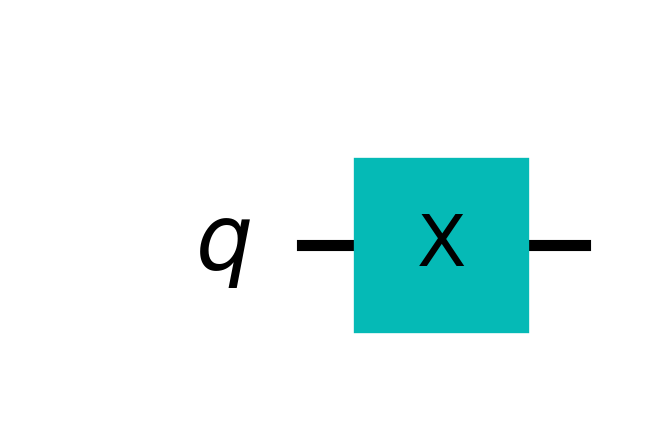
\includegraphics[width=\linewidth]{circuit-depth-1.png}
        \caption*{Circuit depth: 1}\label{fig:circuit_depth_1}
    \end{minipage}
    \hfill
    \begin{minipage}{0.3\linewidth}
        \centering
        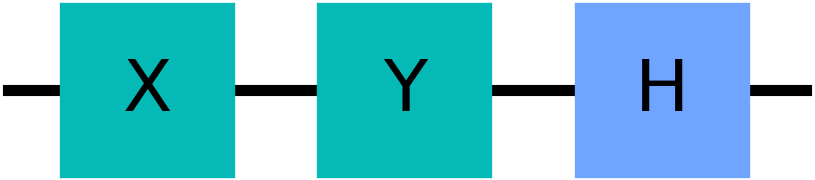
\includegraphics[width=\linewidth]{circuit-depth-3.png}
        \caption*{Circuit depth: 3}\label{fig:circuit_depth_3}
    \end{minipage}
    \hfill
    \begin{minipage}{0.45\linewidth}
        \centering
        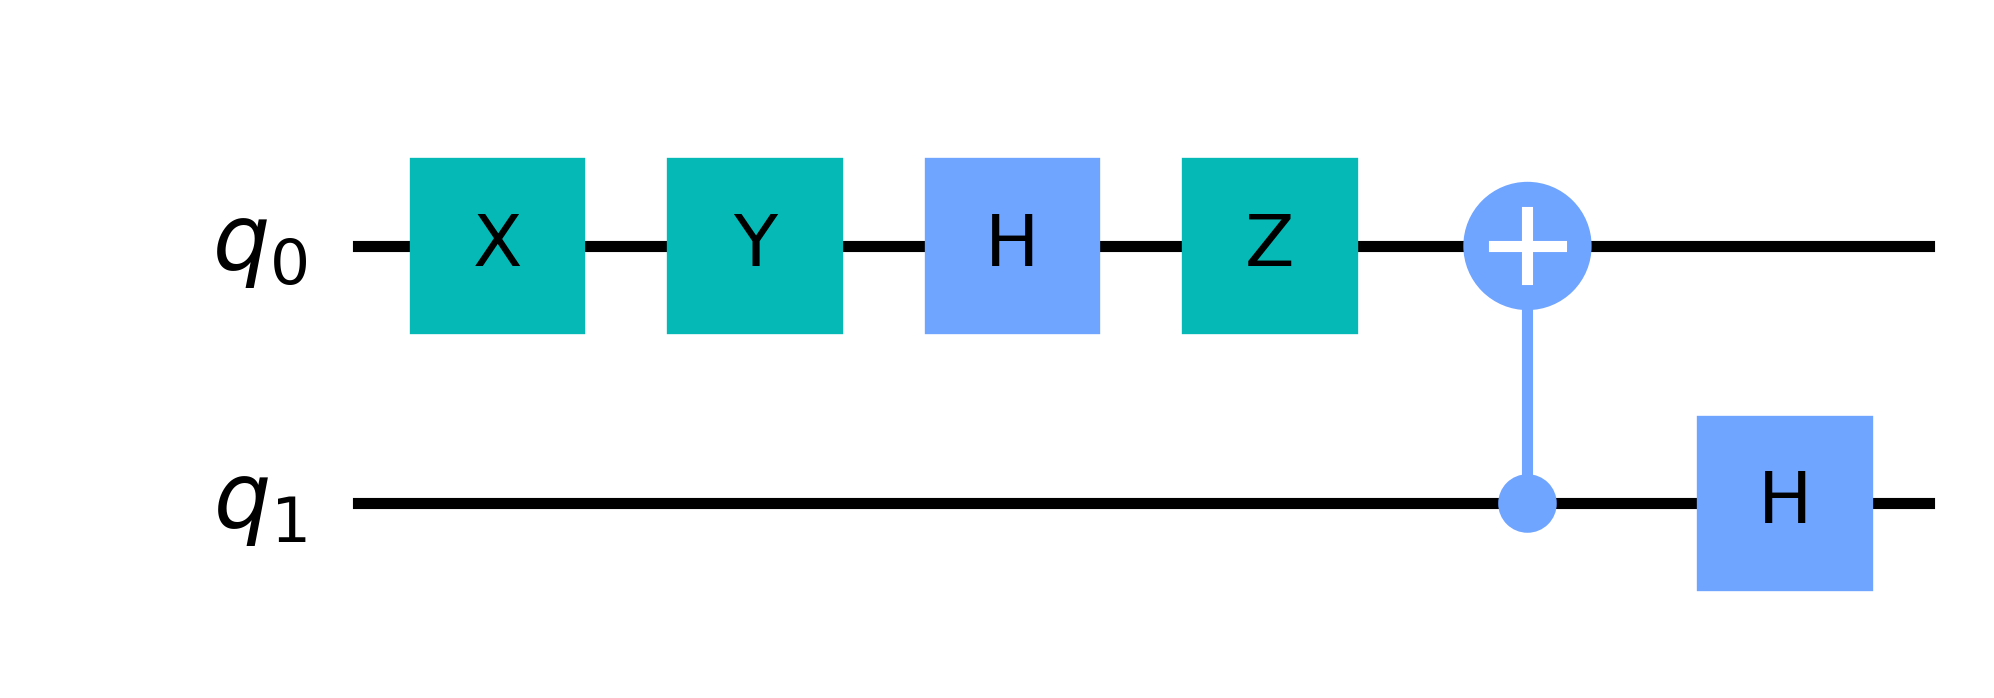
\includegraphics[width=\linewidth]{circuit-depth-6.png}
        \caption*{Circuit depth: 6}\label{fig:circuit_depth_6}
    \end{minipage}
    \caption{Circuit depth}
\end{figure}
\todo{fix sizes of gates and center subcaptions vertically}
Alternatively, we can say it is the longest path in a circuit. Circuits whose depth $\in O(\log n)$ are said to be shallow.
\todo{cite that claim}

\section{Types of ansatzes}
There is a plethora of ansatzes. We will describe the most popular approaches. Broadly we can classify them into two categories: problem inspired and hardware inspired. In addition to that, if ansatz leverages a structure of a particular problem, is said to be problem-specific/problem-derived, otherwise it is problem-agnostic/general. 

\subsection{Hardware efficient ansatz (HEA)}
A problem-agnostic ansatz designed with respect to hardware constraints. Minimizes the number of circuit depth, the number of gates, and entangling qubits in such a way it can be easily implemented on real hardware and thereby tries to minimize error, noise and decoherence.

The structure of HEA consists of layers, each layer consists of rotation gates and entangling gates. In a single layer, we can add multiple levels of rotations using different gates. The final layer does not contain any entangling gates, only rotation gates.

\todo{maybe cite that article that claims to have trainability guarantees on a HEA}\\
\todo{maybe drawbacks, may be very expressive --> difficult to find params}\\
\todo{create a picture which clearly shows the part of layers and the final rotation gates}\\

The fact whether an ansatz is hardware efficient heavily depends on the hardware we are using. We will explain this in the next section.

\subsubsection{Qubit topology and transpilation}
\todo{consider to move it somewhere else}
To enhance the understanding of the hardware-efficient ansatz, we will now explore the specifics of IBM hardware in more detail. IBM has many quantum computers with various qubit counts, topology, and native gate sets. The qubit topology shows qubit connectivity. Upon observation of the qubit topology depicted in Figure \ref{fig:qubit_topology}, it becomes apparent that certain qubits are disconnected and situated far from one another. One might ask how to implement a two-qubit gate between these qubits.

In order to implement a 2-qubit gate between qubits in a quantum circuit that are not directly connected on a quantum device, one or more swap gates must be inserted into the circuit to move the qubit states around until they are adjacent on the device gate map. Each swap gate typically represents an expensive and noisy operation to perform. Thus, finding the minimum number of swap gates needed to map a circuit onto a given device, is an important step (if not the most important) in the whole execution process.~\cite{transpiler}

However, finding the optimal swap mapping is hard. In fact, it is in a class of problems called NP-hard, and is thus prohibitively expensive to compute for all but the smallest quantum devices and input circuits. To get around this, by default Qiskit uses a stochastic heuristic algorithm to compute a good, but not necessarily optimal swap mapping.~\cite{transpiler} \ques{is it cited correctly? I took two aforementioned paragraphs from the Qiskit docs}

In addition to problems with connectivity, we need to also deal with gates that are not supported by the hardware. Each processor family has a native gate set. By default, the systems in each family only support running the gates and operations in the native gate set. Thus, every gate in the circuit must be translated (by the transpiler) to the elements of this set \cite{native_gates}.

This process is called circuit transpilation and fortunately, it is handled automatically by Qiskit so we don't have to worry about it. 
\todo{maybe mention that qiskit offers different levels of transpilation/optimization}
\begin{figure}[H]
    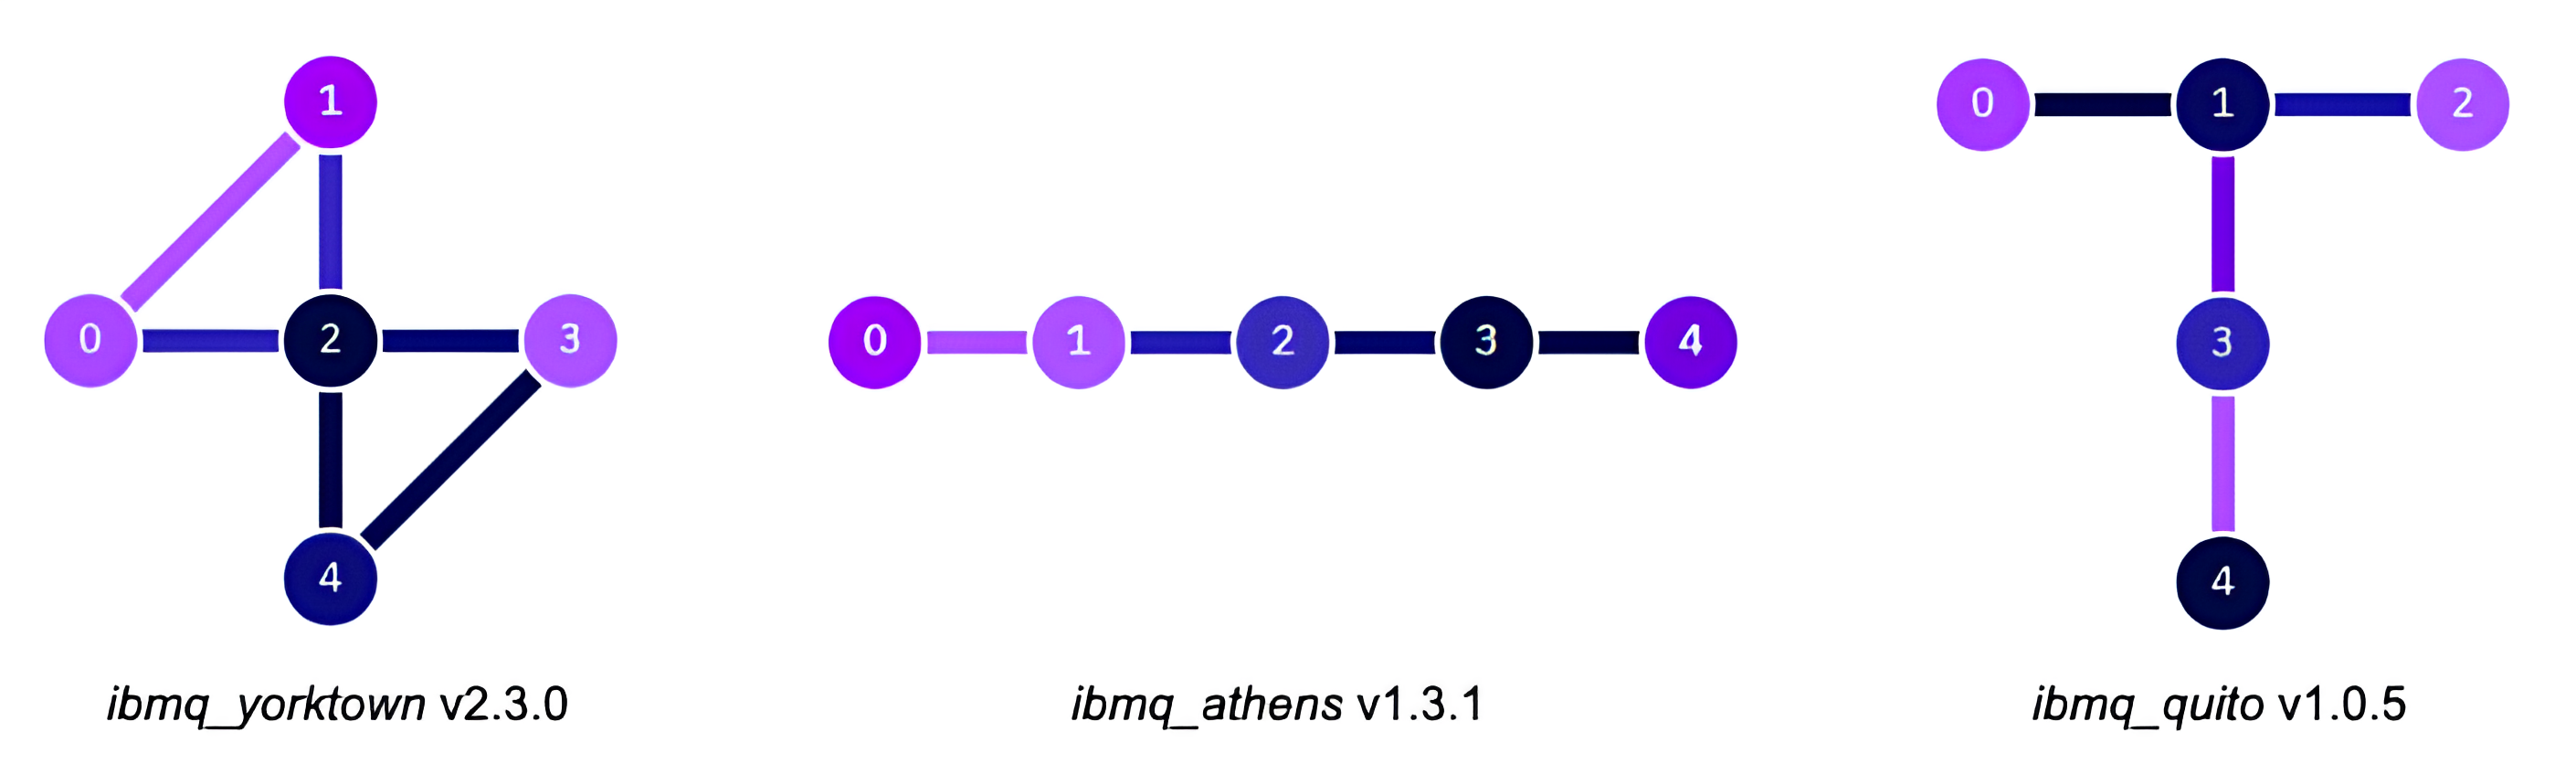
\includegraphics[width=\linewidth]{qubit-topology.png}
    \caption{Example qubit topology of IBM quantum computers}
    \label{fig:qubit_topology}
\end{figure}

\todo{maybe mention entanglement capability}

% https://pennylane.ai/qml/demos/tutorial_here_comes_the_sun/ moze byt useful

\subsection{United Couple Cluster (UCC)}
Unlike HEA, this type of ansatz does not take into account any hardware constraints. It is a chemistry-inspired ansatz proposed for finding a ground state energy of molecules. Despite it being chemistry-inspired, it is still a problem-agnostic ansatz. This seems all good but it suffers from a major drawback. The circuit depth of UCC ansatz grows $O(n^4)$ where $n$ is a number of qubits \cite{ucc_ansatz}. For larger problems and current NISQ devices, this is not feasible due to noise and decoherence, although there are some research endeavors to mitigate this problem.
  
\subsection{Popular ansatzes}

\subsubsection{Full entanglement}
This ansatz entangles each qubit with every other qubit, therefore we hardly can call this ansatz hardware efficient.
\begin{figure}[H]
    
\includegraphics[width=\linewidth]{full-ansatz.png}
    \caption{Ansatz with full entanglement, 2 layers, RY rotation gates}
\end{figure}

\subsubsection{Linear entanglement}
Each adjacent pair of qubits is entangled. 
\begin{figure}[H]
    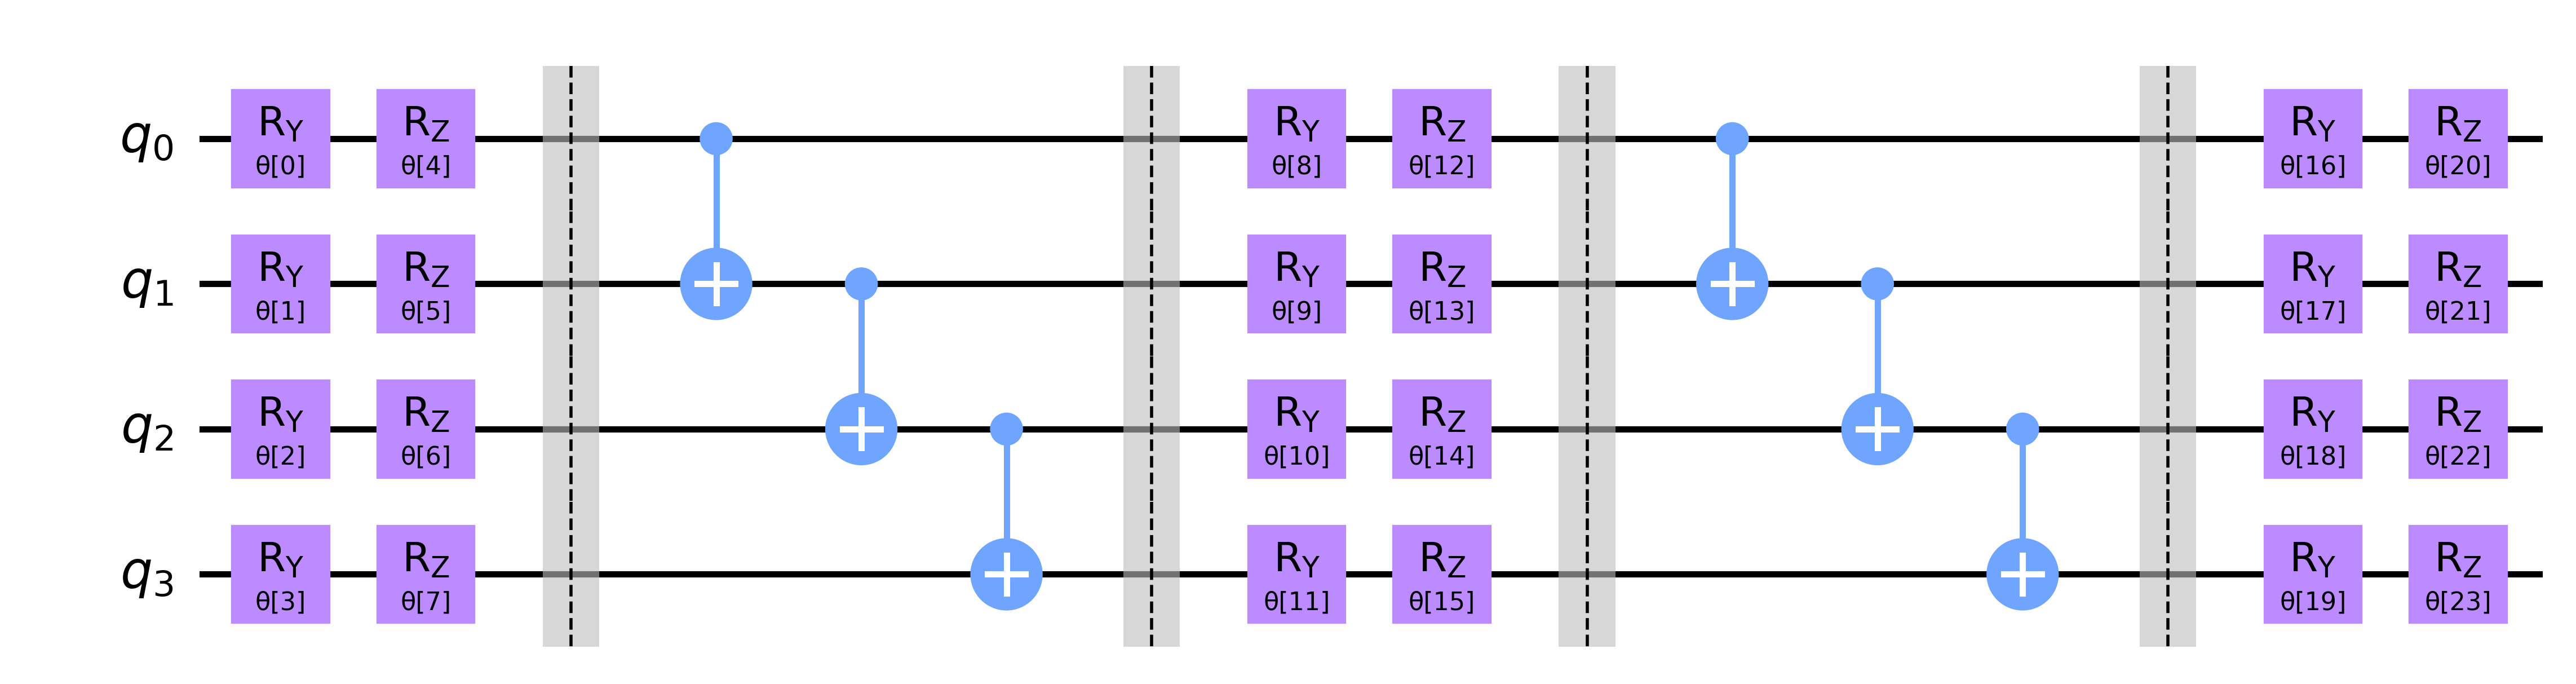
\includegraphics[width=\linewidth]{linear-ansatz.png}
    \caption{Ansatz with linear entanglement, 2 layers, RY rotation gates}
\end{figure}

\subsubsection{Reverse linear entanglement}
Same as linear but in reversed order. Provided the entangling gates are CNOT, this ansatz has the same unitary as full entanglement~\cite{twolocal}. 
\begin{figure}[H]
    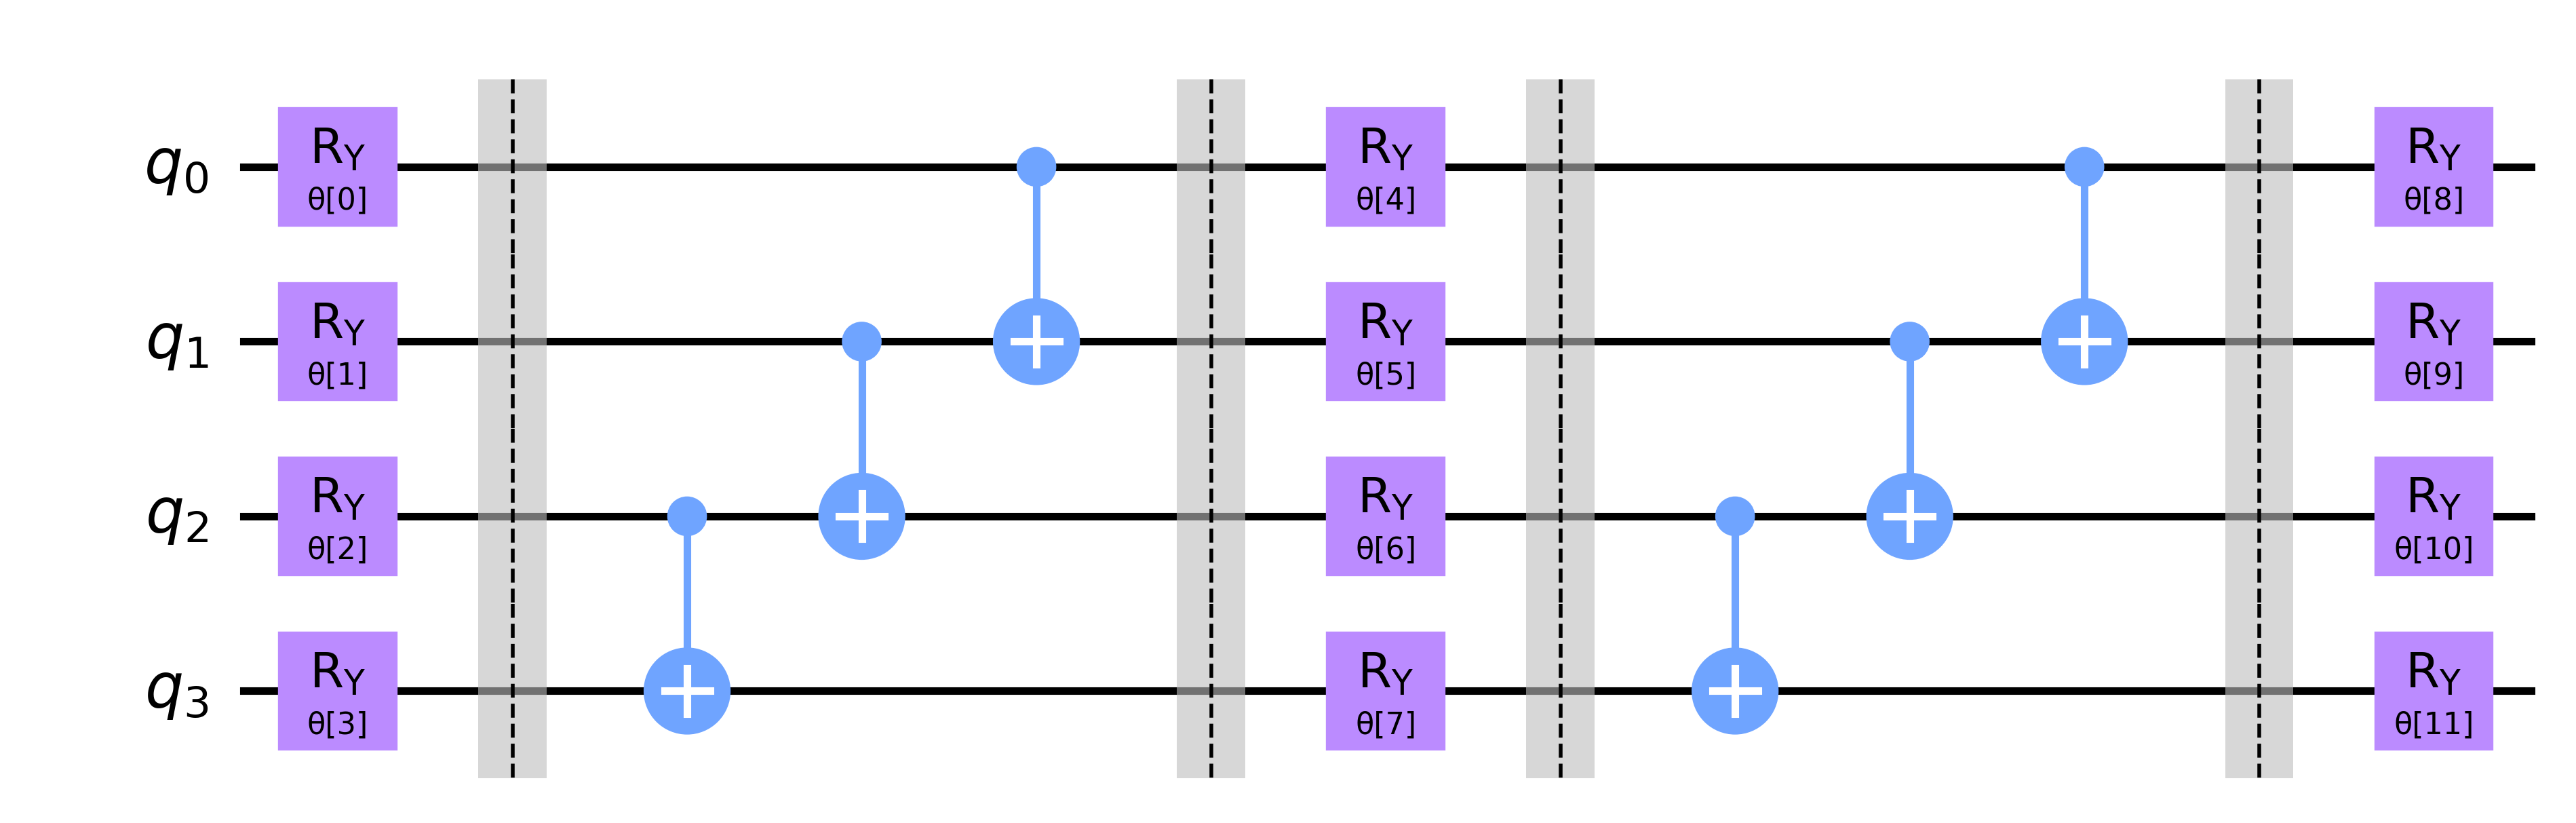
\includegraphics[width=\linewidth]{reverse-linear-ansatz.png}
    \caption{Ansatz with reverse linear entanglement, 2 layers, RY rotation gates}
\end{figure}

\subsubsection{Pairwise entanglement}
Entanglement consists of two ''levels'' where qubit $i$ is entangled with qubit $i+1$ for all even values of $i$, and then a second level where qubit $i$ is entangled with qubit $i+1$ for all odd values of $i$~\cite{twolocal}. 
\begin{figure}[H]
    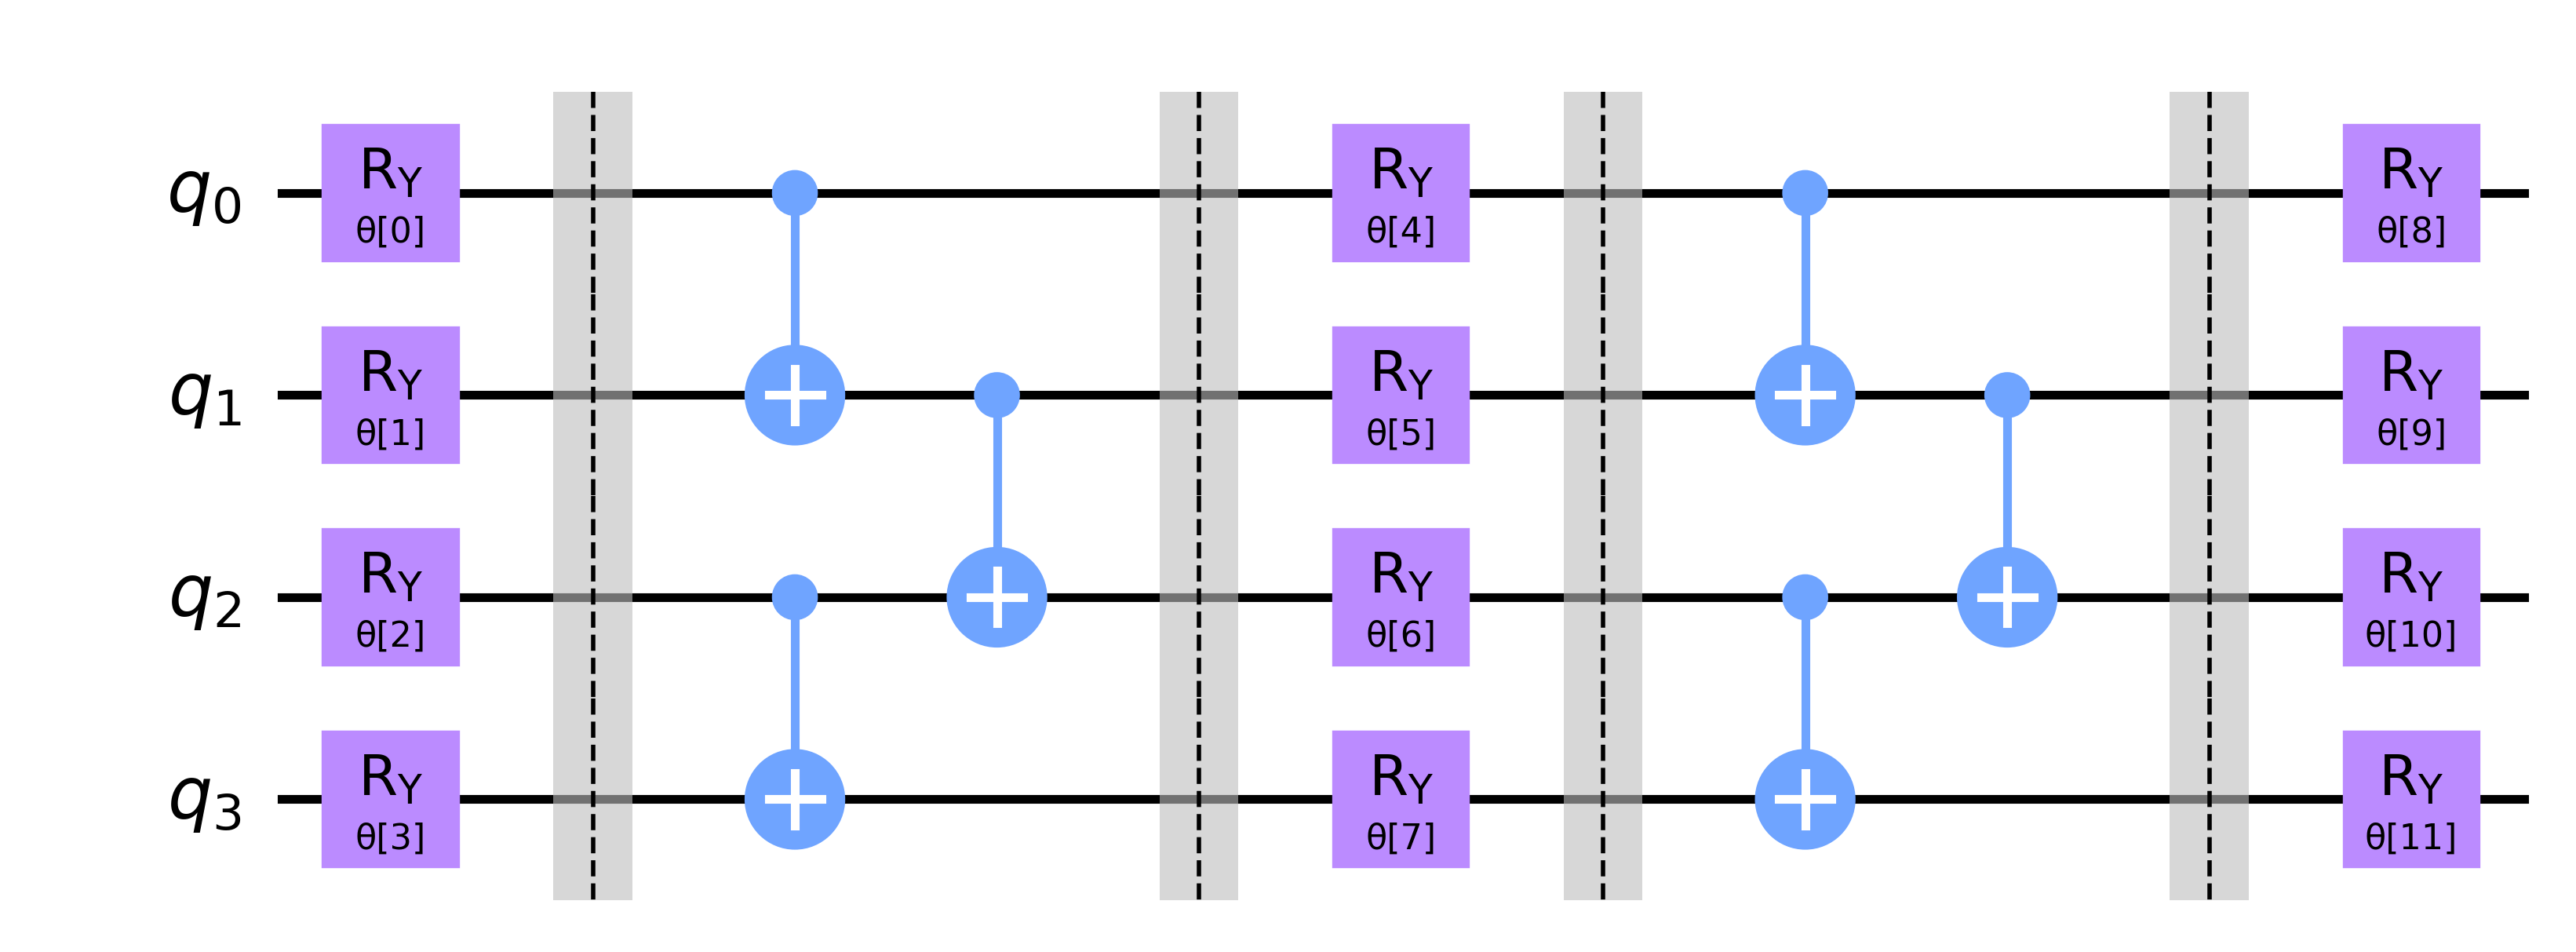
\includegraphics[width=\linewidth]{pairwise-ansatz.png}
    \caption{Ansatz with pairwise entanglement, 2 layers, RY rotation gates}
\end{figure}

\subsubsection{Circular entanglement}
The same as linear but in addition, the last qubit is entangled with the first qubit. In case physical qubits are arranged in a circle, this is easy to implement.
\begin{figure}[H]
    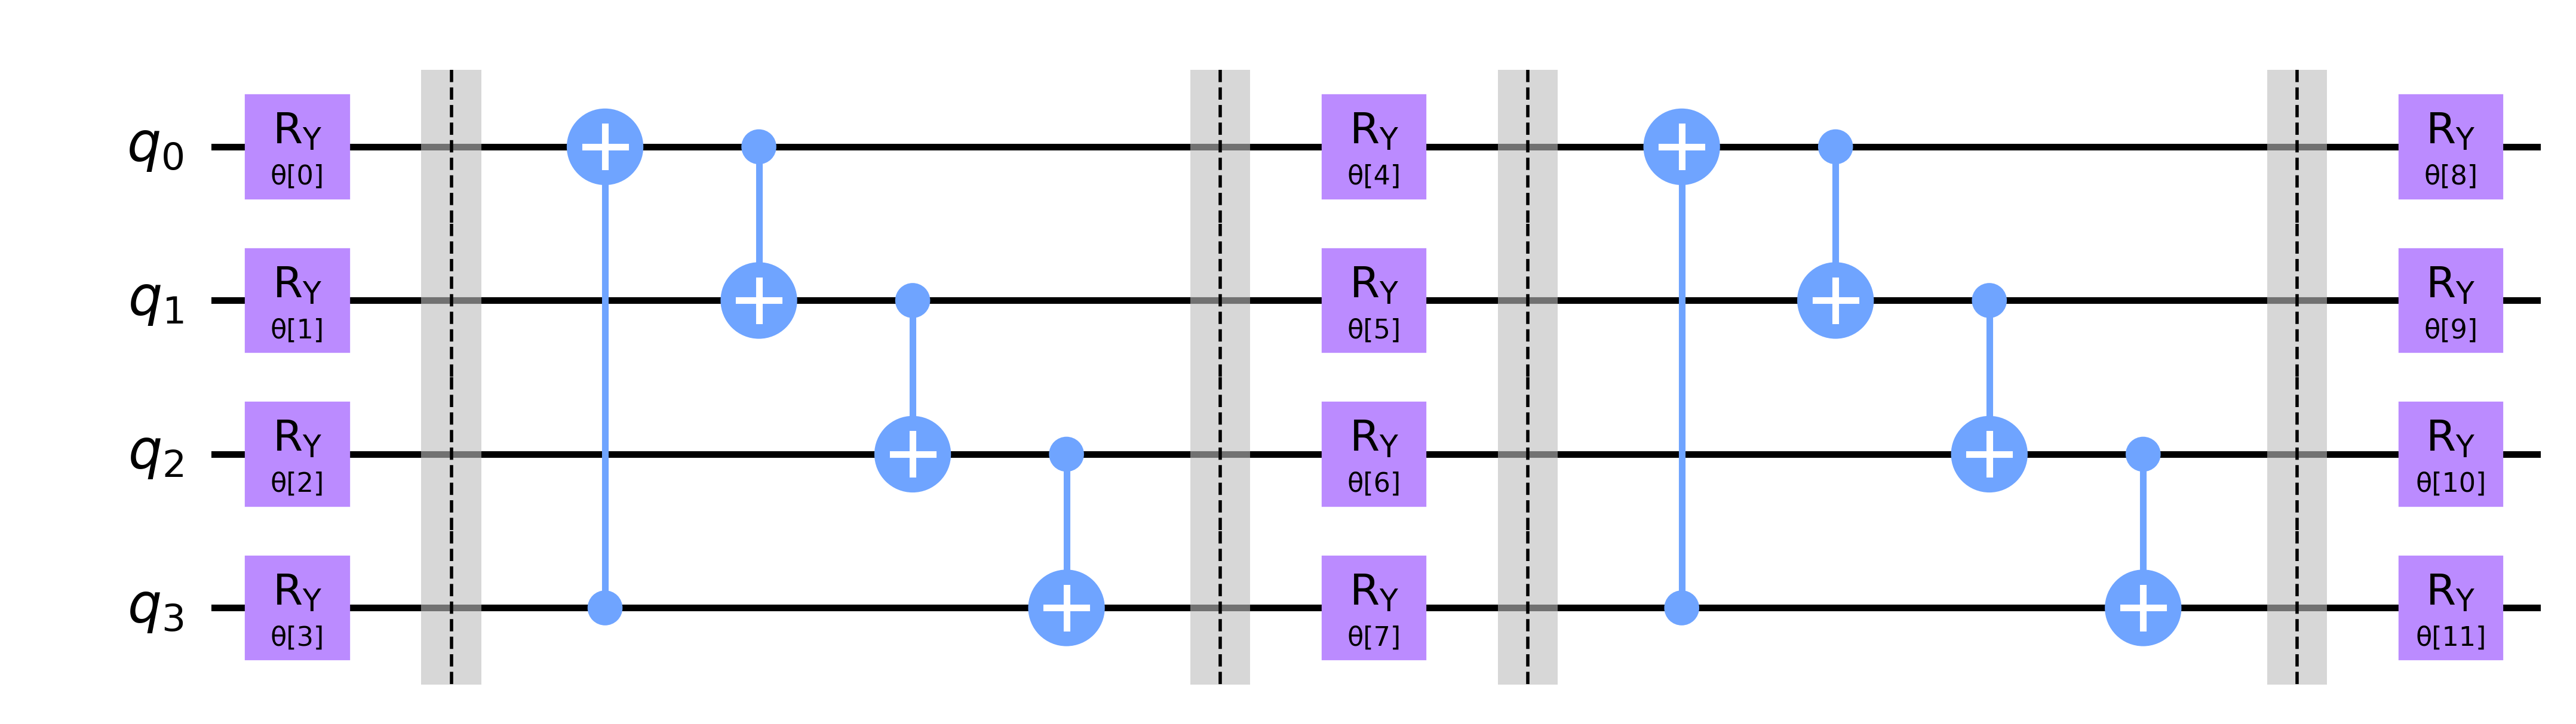
\includegraphics[width=\linewidth]{circular-ansatz.png}
    \caption{Ansatz with circular entanglement, 2 layers, RY rotation gates}
\end{figure}

\subsubsection{Shifted circular alternating (SCA) entanglement}
It consists of circular entanglement where the ''long'' entanglement connecting the first with the last qubit is shifted by one each block. Furthermore, the role of control and target qubits are swapped every block (therefore alternating)~\cite{twolocal}.
\begin{figure}[H]
    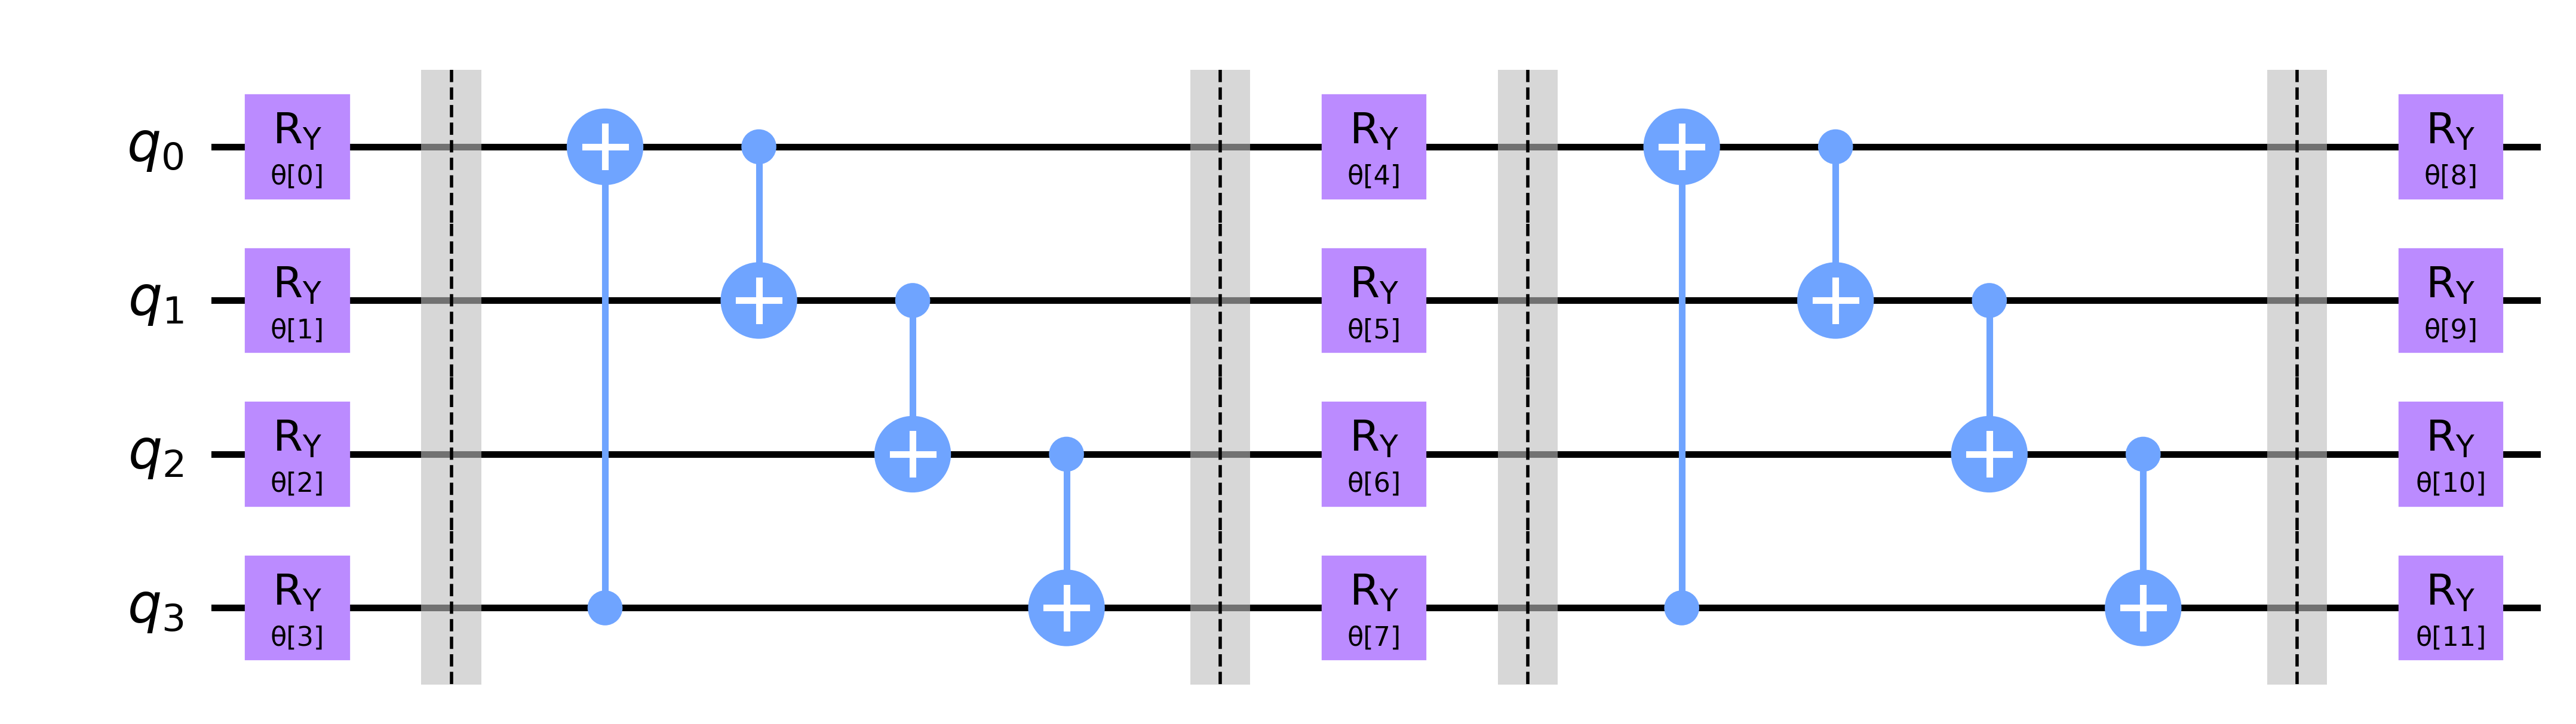
\includegraphics[width=\linewidth]{circular-ansatz.png}
    \caption{Ansatz with shifted circular alternating entanglement, 2 layers, RY rotation gates}
\end{figure}

\todo{play with scaling of images and make sure all the gates are of the same size...}\\

\subsection{Properties of an ideal ansatz}
In essence, our main focus is on attaining these characteristics:
\begin{itemize}
    \item spans only the relevant part of the Hilbert space, ideally only where the solution lies
    \item not too many optimization parameters
    \item reduces gates that can introduce noise
\end{itemize}